\chapter{Previous Solutions}\label{ch:PrevSol}
To understand the concept of social robots and how they work with and around humans it can be beneficial to look into how these robots have previously been implemented. Looking at these robotic proposals can help highlight some of the necessities as well as common issues when implementing a social robot. The findings from these projects will be a starting point of research for this project to develop a social robot for assisting humans in a hypermarket.

\section{Care-O-Bot}\label{sec:cob4}
Care-O-Bot, as seen in figure \ref{fig:cob4}, is developed at Fraunhofer Institute for Manufacturing Engineering and Automation in Germany. It is a mobile robot that is used to assist humans in semi-structured environments. It is built to be used in research areas and to support people in their daily life in a variety of situations. The development of Care-O-Bot began in 1998 and version 4 was released in 2015 \cite{cob4}.

\begin{figure}[H]
    \centering
    \begin{minipage}[b]{0.52\linewidth}
        Care-O-Bot 4 is designed to be configured for specific situations, where an arm or two can be attached to it. The modularity extends to having spherical joints in the neck and hips which allows for 360 degrees of rotation in head and torso, respectively. The design of the robot was based on social role models in order to be accepted socially and interact with humans. This was done by considering three levels of human emotional reaction to everyday use when building the robot. These three levels are visceral, behavioural, and reflective which include appearance, pleasure and effectiveness of use as well as self-image, personal satisfaction and memories \cite{cob4}.
    \end{minipage}
    \hspace{0.42cm}
    \begin{minipage}[b]{0.43\linewidth}
        \centering
        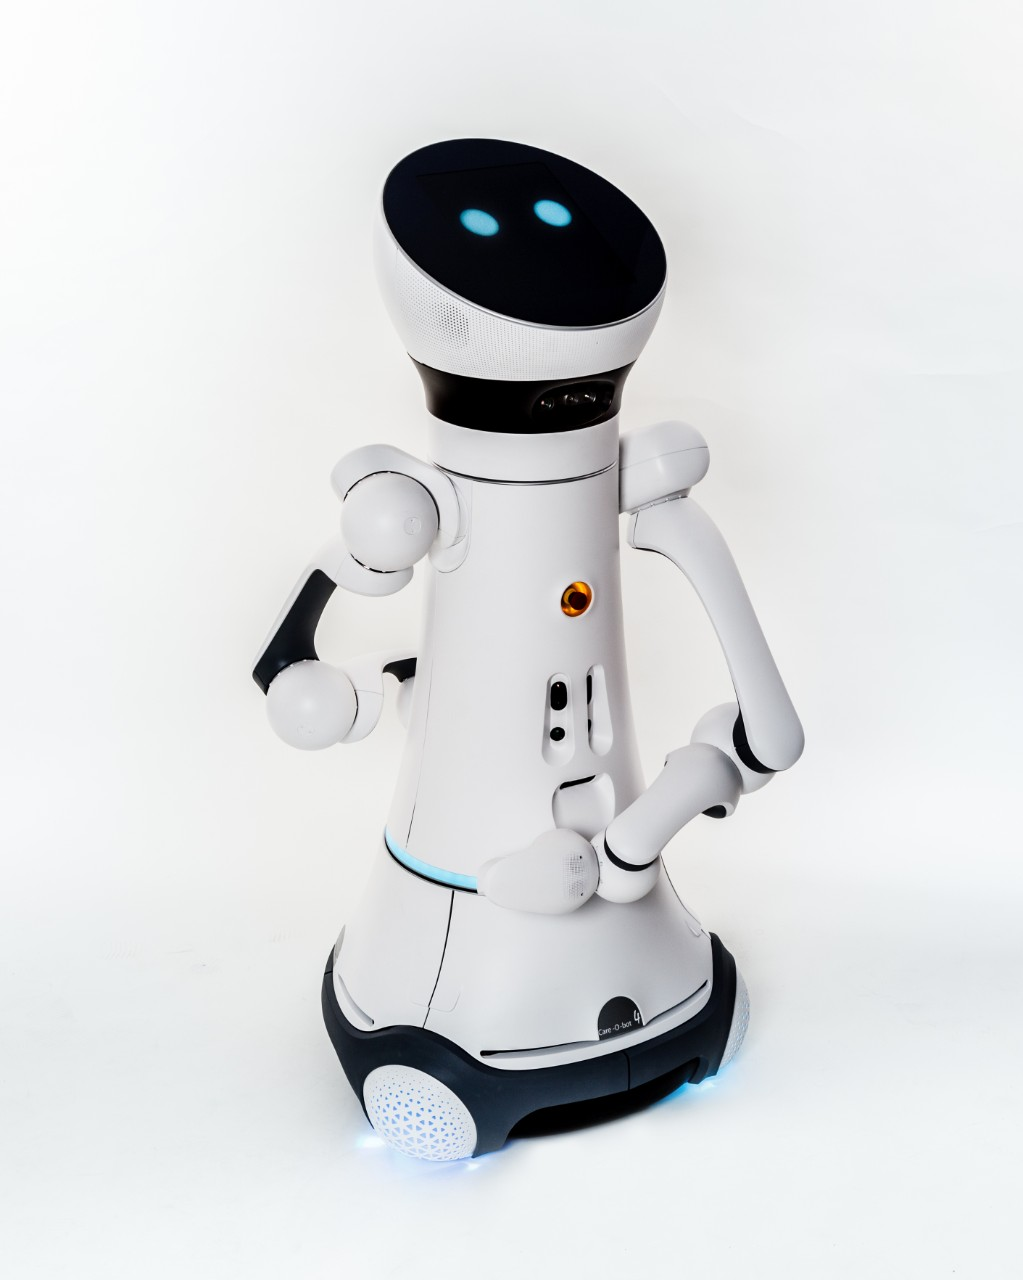
\includegraphics[width=\textwidth]{figures/Cob4.jpg}
        \caption{Care-O-Bot 4 developed by Fraunhofer \cite{cob4_image}.}
        \label{fig:cob4}
    \end{minipage}
\end{figure}

Care-O-Bot 4 is designed to have human features such as posture and natural arm movements. For example, the robot leans forward as a way of showing respect while staying balanced and keeping eye contact. Facial expression, represented by a a pair of eyes, are shown on a touch screen embodied on the robot’s head to express emotions and social cues. The screen is also used to interact with the robot when a user approaches it by showing a graphical user interface. By using the hip and neck joints, the screen can be positioned according to the user's direction \cite{cob4}.

The robot has a microphone that is used to recognise speech, in addition to cameras for recognising persons and hand gestures. Care-O-Bot has speakers and multiple LEDs to indicate the inner state of the robot and a laser pointer to show which object the robot is about to grasp. It is also equipped with 3 laser scanners to avoid obstacles and 3D-RGBD camera in the gripper in order to determine the position of objects \cite{cob4}.


\section{SPENCER}\label{sec:spencer}
SPENCER is a robot assistant, with the purpose of informing and guiding passengers in airports. One of the specific tasks is to bring passengers, travelling with connecting flights, from their arrival gate to the passport control. SPENCER learns human social behaviour to plan appropriate actions in real-time\cite{SPENCER_paper}.
%photo

\begin{figure}[H]
    \centering
    \begin{minipage}[b]{0.485\linewidth}
        SPENCER is designed with a human-inspired abstract appearance, as seen figure \ref{fig:SPENCER_design}. It should look human-like to not appear as unfriendly or threatening, which is an important factor when a robot is interacting with humans, but also not too much like a human, which can lead to disappointment or refusal of the system. This concept is elaborated in section \ref{sec:Psychology}.
        As seen on figure \ref{fig:SPENCER_design}, the robot has a round head with two eyes and mouth in the shape of a smile, making it appear friendly.
        To physically interact with the user, the robot has a touchscreen and a scanner for boarding pass. The sensors in SPENCER consists of two SICK LMS 500 2D laser scanners, multiple RGB-D cameras and a stereo camera system.
    \end{minipage}
    \hspace{0.2cm}
    \begin{minipage}[b]{0.48\linewidth}
        \centering
        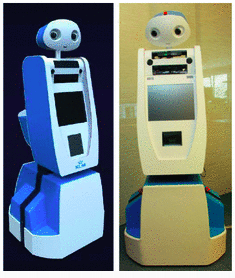
\includegraphics[width=\textwidth]{figures/SPENCERpic.png}
        \caption{Design view and actual appearance of SPENCER robot\cite{SPENCER_paper}. An EU funded research project, tested for KLM in Amsterdam Schiphol airport to manage the passengers flow \cite{SPENCERCITE}. }
        \label{fig:SPENCER_design}
    \end{minipage}
\end{figure}

As a middle-ware for the software components, ROS is used\cite{SPENCER_paper}.
The data from the 2D laser data is used for detecting people. The robot will detect people and divide them into multiple groups. After forming groups, the robot can determine what group of people is interacting with it and who is in need of guidance. %They compute features for segments from the data and classified.
As long as one member is following SPENCER, it is considering the group as following.\\

The robot is using algorithms for both mapping the environment and calculating the probability of the direction of dynamic objects, which is used to predict the direction of moving objects. When planning the route, it is needed to take the social rules into consideration. The robot should not cross through another group of people, but deviate it, when moving to the destination. This is why SPENCER uses a human-aware cost map that makes a path around the group of people detected and SPENCER also moves in a path avoiding abrupt motions by anticipating future collisions and adapting the velocity accordingly\cite{SPENCER_paper}.


\section{Intelligent Shopping Trolley}\label{sec:IST}
The Intelligent Shopping Trolley (IST) is an intelligent system to notify costumers of deals and scheduling the shortest obstacle-free path for the user.
The paper \ref{fig:trolleyRep} states that the real-time communication with the costumer helps with detection of preferences and gives feedback, which can assist them in their daily shopping. Where the real-time communication is a setup of the sensors applied on the trolley to monitor the users behaviour, such as stopping or walking by a specific product. This data is then sent back to the retailer so that they can spectate the results of the costumers using the trolleys and have a real-time communication with them.\\

The solution is run through a system where routers has been set up in each product shelf of the hypermarket, as seen in figure  \ref{fig:trolley2}. Whenever the person passes a sale the trolley will alert the user about the current sales that he or she is passing. The IST also directs the user to the desired products that they need and the conclusion is that the IST users benefit from non-time consumption when using the routes laid out for them.\\
\\
Two pressure sensors, which can be seen on figure \ref{fig:trolley1}, is used to determine whether the trolley is being used or not. The grip of a person exerts a pressure that results in increase in voltage and hereby it can be detected. If the customer leaves the trolley for more than 30 minutes, the trolley is treated as unused and the server will notify an employee to retrieve that trolley.
A G-sensor is used to determine the acceleration of the trolley, and to determine the aforementioned, if the user is stopping at certain wares. The trolley is connected with a module, that wireless connects the trolley with the routers.\\
The overall idea of how the IST system works can be seen on figure \ref{fig:trolleyRep}.

\begin{figure}[H]
    \begin{minipage}[b]{0.5\linewidth}
        \centering
        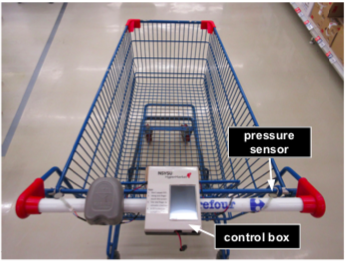
\includegraphics[width=\textwidth]{figures/ISTTrolley.png}
        \caption{The IST system showing where the pressure sensor and the control box is placed\cite{wangintelligent}}
        \label{fig:trolley1}
    \end{minipage}
    \begin{minipage}[b]{0.5\linewidth}
        \centering
        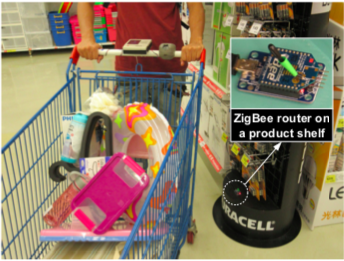
\includegraphics[width=\textwidth]{figures/ISTTrolley2.png}
        \caption{The IST system showing where the wireless router is placed on a product shelf\cite{wangintelligent}}
        \label{fig:trolley2}
    \end{minipage}
\end{figure}

The interaction between the user and the trolley happens through an LCD touch panel in the control box as seen in figure \ref{fig:trolley1}. The customer can search for the location of specific products, and as a result, the shortest obstacle-free path will be provided for the customer. In addition, information such as promotions and products on sale is also shown on the LCD screen.\cite{wangintelligent}.

\begin{figure}[H]
    \centering
    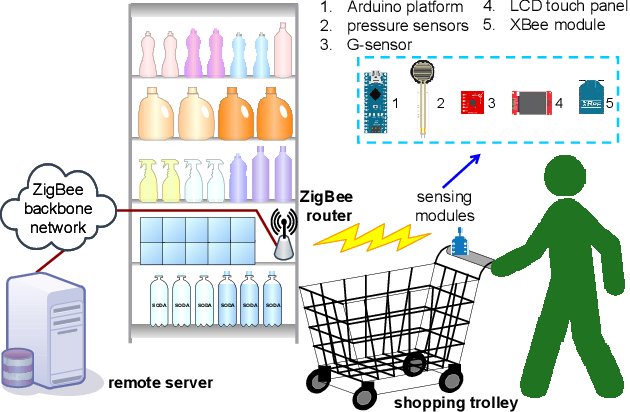
\includegraphics[width=0.75\textwidth]{figures/trolley.png}
    \centering{\caption{A representation of an intelligent trolley \cite{wangintelligent}}\label{fig:trolleyRep}}
\end{figure}

%The path-planning consists of a modified A* algorithm.
The servers can determine where all of the trolleys are positioned, which is used when planning a route to a desired product, so a customer would not collide with another trolley. The server can also analyse and record the customer's behaviour in the retailer's database. This data can be used for determining product shelves that have been visited more often, finding the potentially popular products \cite{wangintelligent}.
\\
\\
%End of chapter
These solutions highlight the current approaches to social robots in environments with multiple humans. The findings from these show that it is important to create a robot that can navigate between humans while insuring that it is safe and comfortable for the humans.